% Options for packages loaded elsewhere
\PassOptionsToPackage{unicode}{hyperref}
\PassOptionsToPackage{hyphens}{url}
%
\documentclass[
]{article}
\usepackage{lmodern}
\usepackage{amssymb,amsmath}
\usepackage{ifxetex,ifluatex}
\ifnum 0\ifxetex 1\fi\ifluatex 1\fi=0 % if pdftex
  \usepackage[T1]{fontenc}
  \usepackage[utf8]{inputenc}
  \usepackage{textcomp} % provide euro and other symbols
\else % if luatex or xetex
  \usepackage{unicode-math}
  \defaultfontfeatures{Scale=MatchLowercase}
  \defaultfontfeatures[\rmfamily]{Ligatures=TeX,Scale=1}
\fi
% Use upquote if available, for straight quotes in verbatim environments
\IfFileExists{upquote.sty}{\usepackage{upquote}}{}
\IfFileExists{microtype.sty}{% use microtype if available
  \usepackage[]{microtype}
  \UseMicrotypeSet[protrusion]{basicmath} % disable protrusion for tt fonts
}{}
\makeatletter
\@ifundefined{KOMAClassName}{% if non-KOMA class
  \IfFileExists{parskip.sty}{%
    \usepackage{parskip}
  }{% else
    \setlength{\parindent}{0pt}
    \setlength{\parskip}{6pt plus 2pt minus 1pt}}
}{% if KOMA class
  \KOMAoptions{parskip=half}}
\makeatother
\usepackage{xcolor}
\IfFileExists{xurl.sty}{\usepackage{xurl}}{} % add URL line breaks if available
\IfFileExists{bookmark.sty}{\usepackage{bookmark}}{\usepackage{hyperref}}
\hypersetup{
  pdftitle={Fantasy Football Modelling with JAGS and Random Forest},
  hidelinks,
  pdfcreator={LaTeX via pandoc}}
\urlstyle{same} % disable monospaced font for URLs
\usepackage[margin=1in]{geometry}
\usepackage{graphicx,grffile}
\makeatletter
\def\maxwidth{\ifdim\Gin@nat@width>\linewidth\linewidth\else\Gin@nat@width\fi}
\def\maxheight{\ifdim\Gin@nat@height>\textheight\textheight\else\Gin@nat@height\fi}
\makeatother
% Scale images if necessary, so that they will not overflow the page
% margins by default, and it is still possible to overwrite the defaults
% using explicit options in \includegraphics[width, height, ...]{}
\setkeys{Gin}{width=\maxwidth,height=\maxheight,keepaspectratio}
% Set default figure placement to htbp
\makeatletter
\def\fps@figure{htbp}
\makeatother
\setlength{\emergencystretch}{3em} % prevent overfull lines
\providecommand{\tightlist}{%
  \setlength{\itemsep}{0pt}\setlength{\parskip}{0pt}}
\setcounter{secnumdepth}{-\maxdimen} % remove section numbering

\title{Fantasy Football Modelling with JAGS and Random Forest}
\author{}
\date{\vspace{-2.5em}2021-01-13}

\begin{document}
\maketitle

\hypertarget{pseudo-poisson-maximum-likelihood-estimation-instead-of-a-log-transformation-for-regression-data-containing-zeroes}{%
\section{Pseudo Poisson Maximum Likelihood Estimation Instead of a Log
Transformation for Regression Data Containing
Zeroes}\label{pseudo-poisson-maximum-likelihood-estimation-instead-of-a-log-transformation-for-regression-data-containing-zeroes}}

In many modelling problems the relationship between the dependent and
independent variables is a log-linear relationship, however if the
dependent variable contains zero values then it is not possible to apply
the log function. There are many datasets where this problem may occur
in practice, for example a wind turbine may produce zero energy in
certain conditions or a seasonal product may have zero sales in a period
of time.

There are a number of commonly suggested solutions to the log function
being undefined at zero. One solution is to remove the zero entries,
this may be reasonable if there are few zeroes and they are zero at
random, however if this is not the case then we may introduce bias into
the estimates of the model coefficients. Another solution is to add a
small number to each value of the dependent variable, and then apply the
log function to a now strictly positive set of numbers. This latter
approach may also bias the coefficient estimates because the log
function is not linear and therefore the relationship with the
independent variables may be impacted differently for small and large
dependent values.

In this note we examine the bias introduced by applying a log
transformation to the dependent variable plus a small constant, and an
alternative solution using a Pseudo Poisson Maximum Likelihood model.

More precisely, suppose that we have observations
\[Y = \{y_1, \ldots, y_n \}\] that we believe have a log-linear
relationship with indepedent variables \[X = \{ x_1, \ldots, x_n \}\],
and that some of \emph{Y} are zero. By adding a small constant, we are
able to take a log transformation and then our model becomes
\[  \log \left( y_i + \delta \right) = \beta_0 + \beta_1 x_i + \epsilon_i \quad i = 1, \ldots, n  \]
where \[\epsilon_i \sim N(0, 1)\].

The alternative method is by using an exponential transformation that
does not require adding a constant to each observation:
\[ y_i = \exp \left( \beta_0 + \beta_1 x_i + \epsilon_i \right) \quad i = 1, \ldots, n . \]
This ``distribution'' is known as a Quasi Poisson distribution; it is
not a real distribution but we can still calculate estimates of the
model coefficients.

There exist a number of statistical packages that allow us to fit a
regression model using the Pseudo Poisson distribution. Here, we use the
\emph{glm} package in R by setting the family to Pseduo Poisson with a
log link function.

The Pseduo Poisson distribution is primarily used to model
over-dispersion in count data, when the assumption of equality in the
mean and variance is not reasonable and the Poisson distribution is no
longer appropriate. The Quasi Poisson distribution estimates the
variance as a linear function of the mean, and is considered an
alternative to the negative Binomial distribution for over-dispersed
count data. In the regression framework assumed in this note, the Pseudo
Poisson maximum likelihood method can be applied to any non-negative
data, not just count data.

\hypertarget{simulated-data-example}{%
\subsection{Simulated Data Example}\label{simulated-data-example}}

We simulate data from a log-linear model containing zeroes and show
there is bias in the linear regression fitted to a log transformation of
the observations plus a small constant and that the Pseudo Poisson
Maximum Likelihood model provides more accurate coefficient estimates.

The data-generating model is as follows: \[ y_i = 
\begin{cases} \exp \left( -1 + 2 \cdot x_i + \epsilon_i \right) & \quad \epsilon_i > -0.7 \\
            0 & \text{otherwise.} \end{cases} , \quad i = 1, \ldots, n.
\]

In the first stage, we look at how varying \(\delta\) impacts the bias
in the coefficient estimates. In this case, we fix the sample-size to be
n = 50 and use a Monte Carlo simulation with simulation-size
\(M = 250\). The bias in estimating the coefficient of the relationship
with \emph{x} is shown in Figure

\begin{figure}

{\centering 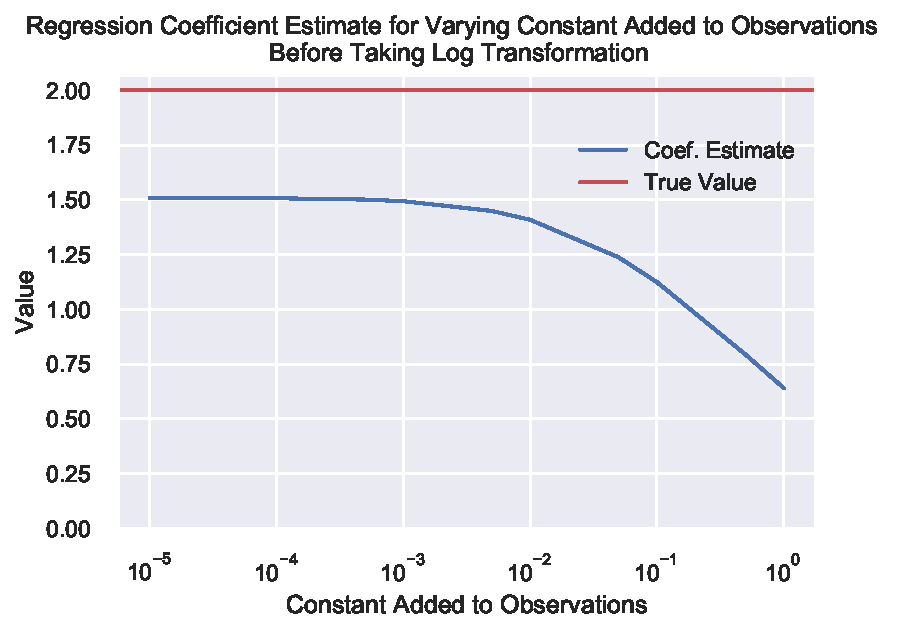
\includegraphics[width=1\linewidth]{D:/Phillip/GitHub/Datasets/Pseudo Poisson Maximum Likelihood/CoefficientBias_withDelta} 

}

\caption{Figure 1: Plot Showing the Impact of Adding a Small Constant to the Observations to Apply a Log Transformation for OLS Regression}\label{fig:unnamed-chunk-1}
\end{figure}

Figure

\begin{figure}

{\centering 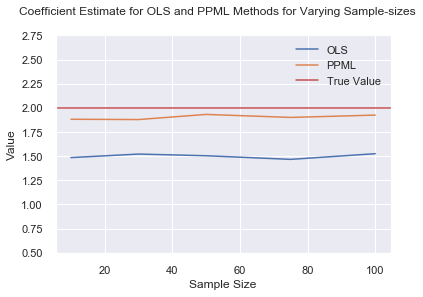
\includegraphics[width=1\linewidth]{D:/Phillip/GitHub/Datasets/Pseudo Poisson Maximum Likelihood/CoefficientBias_samplesize} 

}

\caption{Figure 2: Plot Comparing OLS and Pseudo Poisson Maximum Likelihood for Regression in a Log-Linear Relationship with Zeroes in the Observations}\label{fig:unnamed-chunk-2}
\end{figure}

\end{document}
